\chapter{Model predictive control}
\label{ch:mpc}
In this chapter, the framework conditions of the MPC are described by answering the questions: (i) what is controlled? (ii) How is controlled? (iii) Which curves are controlled? (iii) What data are used? Also, the constraints, the cost function, and the workflow of the MPC script are introduced. The objective of this investigation is to obtain a control signal for the heat pump of the reference building that considers grid services and occupancy comfort. There, the investigation stays in a simulation environment. \newline

\section{Framework conditions of the MPC}
\label{section:FrameworkMPC}
The objective of the MPC is to optimise the control signal of the reference building $\mathbf{u} = (u_1 \enspace u_2)^T = (\dot{Q}_\text{heating} \enspace \dot{Q}_\text{HP})^T$. Thereby, we consider the heat flows of the building in the MPC simulation but, we calculate with a characteristic diagram of the heat pump the electrical control signal $P_\text{HP}$ later. The controlled output is the inside temperature $\mathbf{y} = T_\text{inside}$, which we calculate with the thermal model from \autoref{holeModel}. The desired curves of the $\mathbf{y}$ depend on the presents of occupants, which is determined on an occupancy schedule. Past data of the weather and the dynamic price of the electricity $dP$ \nomenclature[P]{dP}{dynamic Price of the electricity } is used for the simulation environment. \newline

\textbf{Characteristic diagram of the heat pump:}\newline
The characteristic diagram of the heat pump is interpolated with the characteristic values specified by the producer \cite{TUM}. We assume an operation at the nominal power of the heat pump. As \autoref{fig:HeatpumpKennfeld} shows, the electrical power $P_\text{HP}$ depends on the outside temperature $T_\text{outside}$ and the required heat flow $\dot{Q}_\text{HP}$. Further, the heat pump can generate negative $\dot{Q}_\text{HP}$ when cooling is desired. The optimisation of the MPC computed the $\dot{Q}_\text{HP}$, and the $T_\text{outside}$ is known at every time step, then the characteristics of the heat pump are used to calculate the $P_\text{HP}$. 
    \begin{figure}[h]
            \centering
            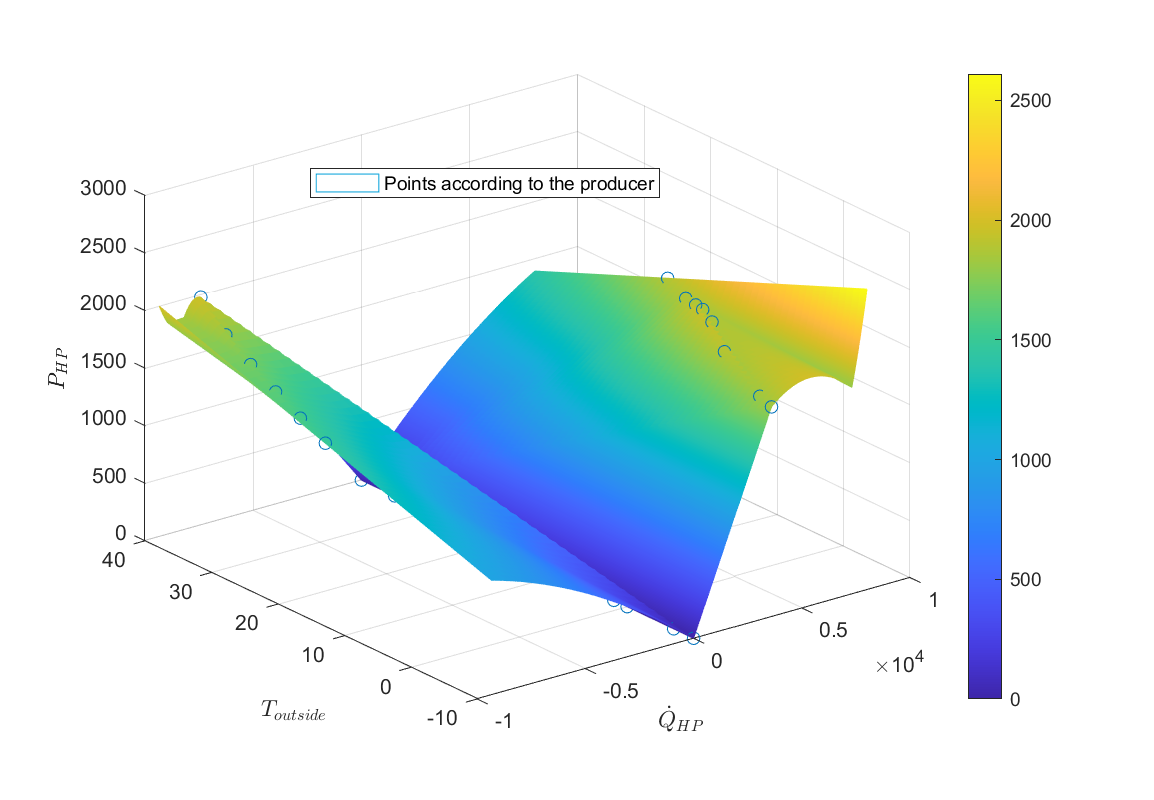
\includegraphics[width=8cm,height=6.5cm]{figure/HeatPumpV55nenn.eps}
           \caption{Interpolation of the characteristic diagram of the heat pump with nominal power according to \cite{TUM}}
           \label{fig:HeatpumpKennfeld}
    \end{figure}
    
\textbf{Occupancy schedule:}\newline
The \autoref{fig:OccupancySchedule} presents the occupancy schedule. It summarises the working time of occupants with a green bar. We assume that persons are in the reference building from Monday to Thursday from 6 am to 7 pm and on Friday from 6 to 6 pm. The assumption is made according to experience values and means that there is a high probability that persons will be in the building during this time.  
    \begin{figure}[h]
            \centering
            
\includegraphics[width=15cm]{figure/Occupancy schedule.PNG}
           \caption{Occupancy schedule of the reference building}
           \label{fig:OccupancySchedule}
    \end{figure}

\textbf{Past data:}\newline
    The data used are from the same period as the training data for the model estimation. As a disturbance variable, we use the recording of diffuse radiation and outside temperature in Energy Lab 2.0. The MPC is simulated over nine days, a little more than a week, to consider the occupancy schedule at least  once.\newline
    The dynamic price of the electricity  $dP$ is made available on the website of the Bundesnetzagentur \cite{Bundesnetzagentur-smard}. Here we use the wholesale prices on the stock exchange as an indicator of grid services. The price is an intersection between supply and demand. Consequently, when the price is low, we can assume an excess of electricity on the grid. It is precisely then that it is particularly suitable to operate our heat pump to obtain electricity from the grid. In the opposite case, the same applies: If the price is high, it is unfavourable to operate the heat pump. At such a time, it is particularly suitable to supply power from the grid. In the opposite case, the same applies: if the price is high, it is unfavourable to operate the heat pump. \newline
    However, negative prices can also arise in retail. Negative prices would undesirably change the costs of the cost function, which will be explained in more detail later at a suitable time. To avoid negative prices, we sum the absolute minimum value of the $dP$ to every value of $dP$. Thus, we shift the curve of $dP$ into positive, as shown in \autoref{fig:Gridverschiebung}.
    \begin{figure}[h]
            \centering
            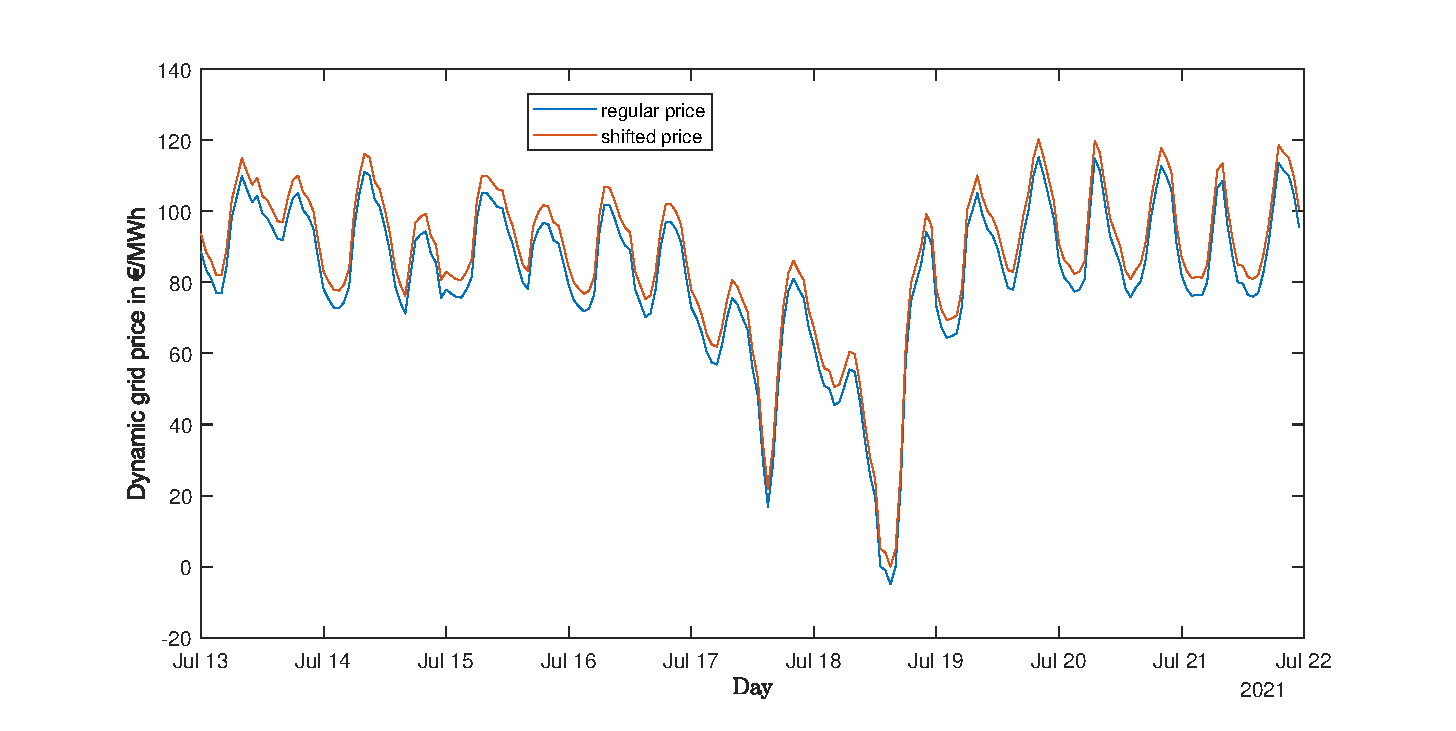
\includegraphics[width=15cm,height=8cm]{figure/Grid_data_Verschiebung.eps}
           \caption{Dynamic price of electricity \cite{Bundesnetzagentur-smard} and shifted dynamic price of electricity}
            \label{fig:Gridverschiebung}
    \end{figure}
    
\section{The Constraints}
\label{section:theconstraints}

The constraints depend on the physical limitations of the installations in the building, such as the heat pump, the underground floor heating, and the water reservoir, or of comfortable reasons. Also, the integration method of the model is included in the constraints. The subsequent section gives an overview of the constraints.\newline

\textbf{Constraints of the control signals:}\newline
The producer's specifications restrict $\dot{Q}_\text{HP}$ the maximum and minimum heat flow of the heat pump for nominal power by heating with the inlet temperature of 55°C and by cooling with the inlet temperature of 18°C \cite{TUM}. The maximum $\dot{Q}_\text{heating}$  is limited according to the underground floor heating calculation, where the set power of every room is counted and we sum it for the complete building \cite{Roth_Auslegung.2020}. The computation of the required cooling power predicts 2246 W needed power by 34.5°C outside temperature in July \cite{SEFIngenieurgesellschaftMBH.2019}. To be more flexible with higher outside temperatures, we round the minimum $\dot{Q}_\text{heating}$ to 2300 W.\newline
Further, we define a constraint to avoid simultaneous heating of building and cooling of the water reservoir or reversed. That would be energy waste. The constraint defines that  % hier noch die ERklärung + in Menge einfügen
The set $\mathbb{U_k}$ summarise mathematically the constraints.
\begin{equation}
    \label{ConstraintU}
    \mathbb{U_k} = \{\mathbf{u_k}| -2300 W \prec \dot{Q}_\text{heating} \prec 5283 W \wedge -9340 W \prec \dot{Q}_\text{HP} \prec 8010 W\} 
\end{equation}

\textbf{Constraints of the states:}\newline
The calculation of the water reservoirs maximal inner energy $U_\text{WR}$ is explained in \autoref{waterModel} with \autoref{eq:max.Energie}. The minimum $U_\text{WR}$ lies by 0 J. The set $\mathbb{X}_{5,k}$ describes the constraint.
\begin{equation}
    \label{ConstraintX5}
    \mathbb{X}_{5,k} = \{x_\text{5,k}| 0 J \prec U_\text{WR} \prec 96370000 J\} 
\end{equation}

\textbf{Constraint of output:}\newline
The Umweltbundesamt \cite{Umweltbundesamt.7.10.2021} recommends an inside temperature of 18°C for some rooms, such as the kitchen. We expand the recommendation to a minimum $T_\text{inside}$ of 18°C for all rooms. The maximum inside temperature refers to the German technical rules for workplaces \cite{Bund.2021}, wherein a maximum of 26°C as room temperature is prescribed. The slack variable $\eta_\text{k}$ allows a variance of the given temperature range during a penalty in the cost function. Thus, we have a soft constraint, and we can obtain the feasibility of the optimisation problem during a deviation of the temperature range \cite{Drgona.2020}. The constraint is represented in the set $\mathbb{Y_k}$ as follows:  
\begin{equation}
    \label{ConstraintX5}
    \mathbb{Y_k} = \{\mathbf{y_k}| 18 \text{°C} - \eta_k \prec T_\text{inside} \prec 26 \text{°C}+ \eta_k\} 
\end{equation}

\textbf{Constraint of heating or cooling:}\newline
%vllt in die Menge von U einschließen
\textbf{Constraint of the integration method:}\newline
The used integration method is the Runge-Kutta method because of its 
\section{The Cost function}
\label{section:thecostfunction}
    \begin{equation}
        \text{minimize} \sum_{k=1}^{N-1} w_\text{1}\cdot (y-y_\text{track})^2 + w_\textbf{2}\cdot(u_\text{2}\cdot dP)^2 + w_\text{3} \cdot \eta^2
    \end{equation}
    %Erklären warum netzkurve verschoben werden musste: positive/neagtives Stellsignal und pos/neg Preis --> Auswrikungen durch quartrierung
    
    %hier erklären, wann gewicht = 0 ist
\section{Workflow of the MPC script}
\label{section:workflowMPC}
\begin{figure}[h]
            \centering
            \def\svgwidth{0.6\textwidth}
            \input{figure/workflowMPC.pdf_tex}
            \caption{Workflow of the MPC script}
            \label{fig:workflowMPC}
    \end{figure}
    
\section{Choice of weightings and horizon}
\label{Choise of weigtings and horizon}